\documentclass[10pt, journal, compsoc]{IEEEtran}

\usepackage{graphicx}
\usepackage{enumerate}
\usepackage{multirow}
\usepackage{fmtcount}
\usepackage{booktabs}
\usepackage{verbatim}
\usepackage[caption=false]{subfig}
\usepackage{hyperref}
\usepackage{flushend}
\usepackage{arydshln}
\usepackage{amsmath}
\usepackage{cases}
\usepackage[nocompress]{cite}
\usepackage[numbers, sort]{natbib}

% For backreferencing footnotes with \cref{label}
\usepackage{cleveref}[2012/02/15]
\crefformat{footnote}{#2\footnotemark[#1]#3}

%For todo notes
\usepackage{color}
\newcommand{\todo}[1]{\colorbox{yellow}{\textbf{[#1]}}}
\newcommand{\revised}[1]{{\color{red}#1}}

% Reduce bibliography font size
\def\bibfont{\footnotesize}

% Reduce space between references
%setlength{\bibsep}{2.5pt}

% Set bibliography title
%\renewcommand\refname{REFERENCES}
%\renewcommand\bibsection{\section{\refname}}

\newcommand{\ea}{{\em et al.}}
\newcommand{\conclusionbox}[1]{%
	\vspace{1mm}
  \noindent
	\framebox[0.48\textwidth][c]{%
		\parbox[b]{0.45\textwidth}{%
			{\em #1}
		}
	}
}

\newcommand{\smallsection}[1]{\subsubsection*{#1}}
\newcommand{\one}{{\tiny $^{*}$}}
\newcommand{\two}{{\tiny $^{**}$}}
\newcommand{\three}{{\tiny $^{***}$}}
\newcommand{\smallnum}[1]{$^{\tiny {\textbf #1}}$}


\newcommand{\rqi}{Do JIT models lose predictive power over time?}
\newcommand{\rqii}{Does the relationship between code change properties and the likelihood of inducing a fix evolve?}
\newcommand{\rqiii}{How accurately do current importance scores of code change properties represent future ones?}

\newcommand{\conjecture}{%
\vspace{0.1mm}
\begin{center}
\parbox[b]{0.4\textwidth}{%
 \centering
{\em Do the important properties of fix-inducing \\
changes remain consistent as systems evolve?}
}
\end{center}
\vspace{0.1mm}
}

\begin{document}

\title{Are Fix-Inducing Changes a Moving Target?\\
{\LARGE A Longitudinal Case Study of Just-In-Time Defect Prediction}}

\author{Shane McIntosh,~\IEEEmembership{Member,~IEEE}
 and Yasutaka Kamei,~\IEEEmembership{Member,~IEEE}%
 \IEEEcompsocitemizethanks{\IEEEcompsocthanksitem S. McIntosh is with the Department of Electrical and Computer Engineering, McGill University, Canada.\protect\\
  Email: shane.mcintosh@mcgill.ca
  \IEEEcompsocthanksitem Y. Kamei is with the Principles of Software Languages Group (POSL), Kyushu University, Japan.\protect\\
  Email: kamei@ait.kyushu-u.ac.jp
 }
}

\IEEEtitleabstractindextext{%
 \begin{abstract}
 Just-In-Time (JIT) models identify fix-inducing code changes.
 JIT models are trained using techniques that assume that past fix-inducing changes are similar to future ones.
 However, this assumption may not hold, e.g., as system complexity tends to accrue, expertise may become more important as systems age.

 \hspace{4mm}
 In this paper, we study JIT models as systems evolve.
 Through a longitudinal case study of 37,524 changes from the rapidly evolving {\sc Qt} and {\sc OpenStack} systems, we find that fluctuations in the properties of fix-inducing changes can impact the performance and interpretation of JIT models.
 More specifically:
 (a) the discriminatory power (AUC) and calibration (Brier) scores of JIT models drop considerably one year after being trained;
 (b) the role that code change properties (e.g., Size, Experience) play within JIT models fluctuates over time;
 and (c) those fluctuations yield over- and underestimates of the future impact of code change properties on the likelihood of inducing fixes.
 To avoid erroneous or misleading predictions, JIT models should be retrained using recently recorded data (within three months).
 Moreover, quality improvement plans should be informed by JIT models that are trained using six months (or more) of historical data, since they are more resilient to period-specific fluctuations in the importance of code change properties.
 \end{abstract}

 \begin{IEEEkeywords}
  Just-In-Time prediction, defect prediction, mining software repositories
 \end{IEEEkeywords}
}

\maketitle

\IEEEdisplaynontitleabstractindextext

\IEEEpeerreviewmaketitle

\IEEEraisesectionheading{\section{Introduction}}
\label{sec:intro}

\IEEEPARstart{T}{he} limited Software Quality Assurance (SQA) resources of software organizations must focus on software modules that are likely to be defective in the future.
To that end, {\em defect prediction models} are trained using historical data to identify defect-prone software modules (e.g., methods~\cite{giger2012esem, hata2012icse}, files~\cite{zimmerman2007}, or subsystems~\cite{nagappan2005icse}).
After being trained using data from historical releases, defect prediction models can be used to prioritize SQA effort according the predicted defect proneness of the modules of a future release.

Change-level defect prediction~\cite{mockus2000bell}, a.k.a., Just-In-Time (JIT) defect prediction~\cite{kamei2013tse}, is an alternative to module-level defect prediction, which has several advantages~\cite{shihab2012fse}.
First, since changes often smaller than modules, JIT predictions are made at a finer granularity, which localizes the inspection process.
Second, while modules have a group of authors, changes have only one, which makes triaging JIT predictions easier (i.e., predictions can be assigned to the author of the change).
Finally, unlike module-level prediction, JIT models can scan changes as they are being produced, which means that problems can be inspected while design decisions are still fresh in the developers' minds.

Despite the advantages of JIT defect prediction, like all prediction models, they assume that the properties of past events (i.e., fix-inducing changes) are similar to the properties of future ones.
Yet, the consistency of properties of fix-inducing changes remains largely unexplored.
It may indeed be the case that the properties of fix-inducing changes in one development period are entirely different from the fix-inducing changes of another.
For example, since complexity tends to accrue as systems age~\cite{belady1976}, expertise may grow more important as systems age.
To that end, in this paper, we set out to address the following central question:

\conjecture

To address our central question, we train JIT models to identify fix-inducing changes using six families of code change properties, which are primarily derived from prior studies~\cite{mockus2000bell, kim2008tse, kamei2013tse, kononenko2015icsme}).
These properties measure:
(a) the magnitude of the change ({\em Size});
(b) the dispersion of the changes across modules ({\em Diffusion});
(c) the defect proneness of prior changes to the modified modules ({\em History});
(d) the experience of the author ({\em Author Experience}) and
(e) code reviewer(s) ({\em Reviewer Experience});
and (f) the degree of participation in the code review of the change ({\em Review}).
Through a longitudinal case study of the {\sc Qt} and {\sc OpenStack} projects, we address the following research questions:

\begin{enumerate}[{\bf (RQ1)}]
\item {\bf \rqi}\\
  \underline{Motivation:}
    If properties of fix-inducing changes do change, JIT models that were trained to identify fix-inducing changes of the past would quickly lose their predictive power.
Hence, we are first interested in (a) whether JIT models lose predictive power over time, and (b) how quickly such losses would occur.

  \underline{Results:}
  After one year, our JIT models typically lose 11--22 and 14--34 percentage points of their discriminatory power (AUC) in the {\sc Qt} and {\sc OpenStack} systems, respectively.
  Similarly, after one year, our JIT models lose up to 11 and 19 percentage points from their calibration (Brier) scores in the {\sc Qt} and {\sc OpenStack} systems, respectively.
  \newpage
\item {\bf \rqii}\\
  \underline{Motivation:}
 Another symptom of changing properties of fix-inducing changes would be fluctuations in the impact that code change properties have on the explanatory power of JIT models.
 If properties of fix-inducing changes do indeed change, the prediction modelling assumption that properties of prior and future events are similar may not be satisfied.
  To cope with this, teams may need to refit their models.
  To better understand how volatile the properties of fix-inducing changes are, we set out to study trends in the importance scores of code change properties in our JIT models over time. 

  \underline{Results:}
  The {\em Size} family of code change properties is a consistent contributor of large importance scores.
  However, the magnitude of these importance scores fluctuates considerably, ranging between 10\%--43\% and 3\%--37\% of the period-specific explanatory power of our {\sc Qt} and {\sc OpenStack} JIT models, respectively.
\item {\bf \rqiii}\\
  \underline{Motivation:}
  Fluctuations in the importance scores of code change properties may impact {\em quality improvement plans}, i.e., team initiatives to reduce the rate of defects, which are based on interpretation of JIT models.
  For example, if a quality improvement plan is formulated based on a large importance score of a property $p$, but $p$ drops in importance in the following period, even a perfectly executed quality improvement plan will have a smaller impact than anticipated.
  On the other hand, if property $p$ has a small importance score in the past, but grows more important in the following period, the quality improvement plan may omit important focal points.
  To better understand the impact that fluctuations have on quality improvement plans, we study the magnitude of these fluctuations in our JIT models.

  \underline{Results:}
The stability of property importance scores in our JIT models is project-sensitive.
The contributions of impactful property families like {\em Size} are both consistently:
(a) overestimated in our {\sc Qt} JIT models by a median of 5\% of the total explanatory power 
and (b) underestimated in our {\sc OpenStack} JIT models by a median of 2\% of the total explanatory power.
\end{enumerate}

Our results lead us to conclude that properties of fix-inducing changes can fluctuate, which may impact both the performance and interpretation of JIT defect models.
To mitigate the impact on model performance, researchers and practitioners should add recently accumulated data to the training set and retrain JIT models to contain fresh data from within the last six months.
To better calibrate quality improvement plans (which are based on interpretation of the importance scores of code change properties), researchers and practitioners should put a greater emphasis on larger caches of data, which contain at least six months worth of data, to smooth the effect of spikes and troughs in the importance of properties of fix-inducing changes.

\subsubsection*{Paper Organization}
The remainder of the paper is organized as follows.
Section~\ref{sec:related} discusses the related work.
Section~\ref{sec:design} describes the design of our case study, while Section~\ref{sec:results} presents the results.
Section~\ref{sec:practice} presents practical suggestions that are informed by our study results.
Section~\ref{sec:threats} discloses the threats to the validity of our study.
Finally, Section~\ref{sec:conclusions} draws conclusions.

\section{Related Work}
\label{sec:related}
\subsection{JIT Defect Prediction}
Some previous studies focus on change-level defect prediction (i.e., JIT defect prediction). For example, Mockus and Weiss~\cite{Mockus2000} predict commits as being buggy or not in an industrial project. They use metric-based features, such as the number of subsystems touched, the number of files modified, the number of lines of added code, and the number of modification requests. Motivated by their previous work, Kamei et al.~\cite{Kamei:2013:LES} built upon the set of code change features, reporting that the addition of a variety of features that were extracted from the Version Control System (VCS) and the Issue Tracking System (ITS) helped to improve the prediction accuracy. They conduct an empirical study of the effectiveness of JIT defect prediction on a set of six open source and five commercial projects and also evaluate their findings when considering the effort required to review the changes.

Aversano \emph{et al.}~\cite{Aversano2007} and Kim \emph{et al.}~\cite{Kim2008} use source code change logs to predict commits as being buggy or not. For example, Kim \emph{et al.}~\cite{Kim2008} used the identifiers in added and deleted source code and the words in change logs. The experimental results on the datasets collected from 12 open source software projects show that the proposed approach achieve 78 percent accuracy and a 60 percent recall.

Kononenko et al.~\cite{Kononenko:2015} found that the addition of code change properties that were extracted from code review databases contributed a significant amount of explanatory power to JIT models. McIntosh and Kamei also 
%\cmt{TODO: update here} 
%The importance of impactful families of code change properties like Size and Review are consistently under/overestimated in the studied systems.

Comparing with these previous studies, we introduce the JIT defect prediction model (DeepJIT) that learn a deep representation of commits and compare the prediction performance of DeepJIT with other JIT models on the dataset including code change properties that are extracted from code review databases. We extended the datasets that McIntosh and Kamei used to analyze~\footnote{\url{https://github.com/software-rebels/JITMovingTarget}} by adding commit messages and code changes. 

\subsection{Deep Learning Models in Defect Prediction}

%Xin Xia's group

%Lin Tang's group

%Say the difference between them and us.
\section{Case Study Design}
\label{sec:design}

In this section, we describe our: (1) rationale for selecting our studied systems and (2) data extraction process. In addition, we describe our approaches to: (3) model construction and (4) model analysis.

\subsection{Studied Systems}
\label{sec:studied}

To address our research questions, we perform a longitudinal case study on successful and rapidly evolving open source systems.
In selecting the subject systems, we identified three important criteria that needed to be satisfied:

\begin{itemize}
  \item {\bf Criterion 1: Traceability.}
    We need reliable data in order to produce healthy datasets (see Section~\ref{sec:related_bias}).
    To that end, it should be reasonably straightforward to extract from the VCS of a studied system, a series of {\em code changes}, i.e., listings of changed lines to a set of code files that developers have submitted to the VCS together.
    It should also be straightforward to connect a large proportion of those code changes to issue reports, which are stored in ITSs, and code review data, which is stored in code review databases.
    Without a traceable process, our code change properties will be unreliable, and our JIT models may be misleading.
  \item {\bf Criterion 2: Rapidly evolving.}
    In order for JIT models to yield the most benefit, our studied systems must undergo plenty of change on a continual basis.
  \item {\bf Criterion 3: Code review policy.}
    Recent studies report that code review can have an impact on post-release software quality~\cite{mcintosh2016emse,thongtanunam2015msr} and defect proneness~\cite{kononenko2015icsme}.
    To control for this, we focus our study on systems where code reviewing is a common practice.
\end{itemize}

In order to address criterion 1, we study systems that adopt the Gerrit code review tool.\footnote{\url{https://code.google.com/p/gerrit/}}
Gerrit tightly integrates with VCSs, automatically submitting commits after project-specific quality gates are passed (e.g., two reviewers vote in favour of acceptance of a change).
These Gerrit-generated commits are accompanied by a structured message, which includes references to the review record (ChangeID) and any addressed issue reports (IssueIDs).

Table~\ref{tab:cases} shows that, similar to our prior work~\cite{mcintosh2016emse, thongtanunam2016emse}, we begin with six candidate systems that adopt the Gerrit code review tool.
In order to address criterion 2, we remove {\sc ITK} from our set of candidate systems because only 3,347 changes appear in the {\sc ITK} Gerrit instance over four years.

In order to address criterion 3, we ensure that the studied systems have high rates of review coverage.
Since we find that only 55\% of {\sc VTK}, 4\% of {\sc Android}, and 14\% of {\sc LibreOffice} changes could be linked to reviews, we remove these three systems from our set of candidate systems.

Table~\ref{tab:cases} provides an overview of the two candidate systems that satisfy our selection criteria ({\sc Qt} and {\sc OpenStack}).
{\sc Qt} is a cross-platform application framework whose development is supported by the Digia corporation, however welcomes contributions from the community-at-large.\footnote{\url{http://qt.digia.com/}}
{\sc OpenStack} is an open-source software platform for cloud computing that is developed by many well-known software organizations (e.g., IBM, VMware, NEC).\footnote{\url{http://www.openstack.org/}}
Although the cleaning process is described below (see Section~\ref{sec:cleaning}), the clean {\sc Qt} dataset contains 25,150 code changes, 23,821 of which (95\%) can be linked to code reviews.
Similarly, the clean {\sc OpenStack} dataset contains 12,374 code changes, 12,041 of which (97\%) can be linked to code reviews.

\subsubsection{Gerrit Code Review Process}

\begin{figure}
  \centering
  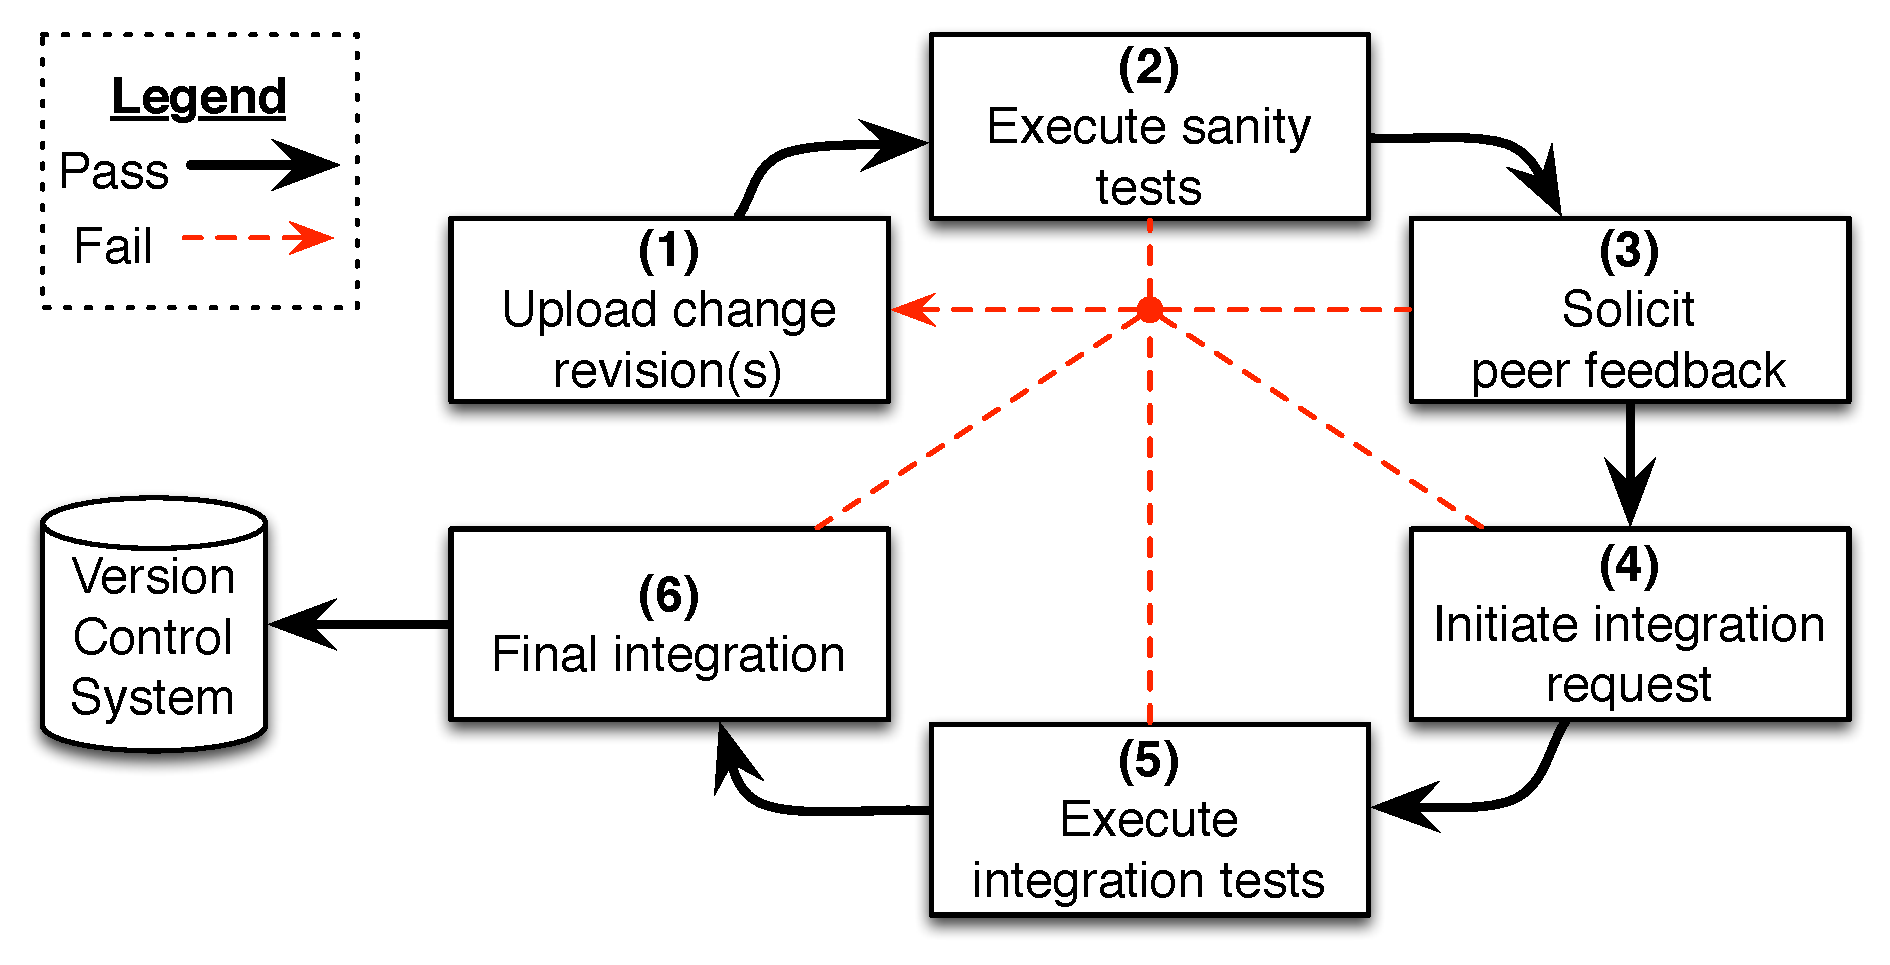
\includegraphics[width=\columnwidth]{figures/contrib_mgmt.pdf}
  \caption{An overview of the Gerrit-based code review process.}
  \label{fig:contrib_mgmt}
\end{figure}

Gerrit is a code review tool that enables a traceable code review process for {\tt git}-based software projects.
It tightly integrates with test automation and code integration tools, allowing users to codify code review and verification criteria that must be satisfied before a code change can be integrated into upstream {\tt git} repositories.

Using Gerrit, both the {\sc Qt} and {\sc OpenStack} projects implement similar workflows for managing code contributions.
Figure~\ref{fig:contrib_mgmt} provides an overview of the process, which is made up of the following steps, checks, and quality gates.

\begin{enumerate}[{\bf (1)}]
    \item {\bf Upload change revision(s).}
      An author of a code change uploads a new change or a change revision to a Gerrit instance and invites a set of reviewers to critique it by leaving comments for (a) the author to address; or (b) review participants to discuss.

    \item {\bf Execute sanity tests.}
      Before reviewers examine the submitted changes, sanity tests verify that the changes are compliant with the coding style conventions, and does not introduce obvious regression in system behaviour (e.g., code does not compile).
      If the sanity tests report issues, the change is blocked from integration until the author uploads a revision of the change that addresses the issues.
      This step provides quick feedback and avoids wasting reviewer effort on finding style or low-level coding issues that can be automatically checked.

    \item {\bf Solicit peer feedback.}
      After the submitted changes pass sanity testing, the author solicits reviewers to examine the change.
      Each reviewer is asked to provide feedback and a review score.
      In Gerrit, reviewers can provide one of five score values:
      ``+2'' indicates strong support for the change and approval for integration,
      ``+1'' indicates weak support for the change without approval for integration,
      ``0'' indicates abstention,
      ``-2'' indicates strong disagreement with the change and also blocks integration, and
      ``-1'' indicates weak disagreement with the change without blocking integration.

    \item {\bf Initiate integration request.}
      Gerrit allows teams to codify code review and verification criteria that must be satisfied before changes can be integrated into the project {\tt git} repositories.
      For example, the {\sc OpenStack} integration policy specifies that an author needs to receive at least two +2 scores.\footnote{\url{http://docs.openstack.org/infra/manual/developers.html\#project-gating}}
      After satisfying the integration criteria, the author can initiate an integration request, which queues the change for integration.

    \item {\bf Execute integration tests.}
      Code changes that are queued for integration are scanned by the integration testing system.
      The integration testing system runs a more rigourous set of tests than the sanity testing phase to ensure that changes that land in the project {\tt git} repositories are clean.
      If the integration tests report failures, the change may not be integrated until the author uploads a revision of the change that addresses the failures.

    \item {\bf Final integration.}
      Once the change passes integration testing, Gerrit automatically commits the change into the upstream (official) project {\tt git} repositories.
  \end{enumerate}

  Table~\ref{tab:cases} shows that the Gerrit-based code review processes of {\sc Qt} and {\sc OpenStack} achieve high coverage rates of 95\% and 97\%, respectively.
  On occasion, the code review process is omitted due to a rush to integrate a critical change.
  However, the vast majority of changes undergo a code review.
  Moreover, changes are rarely approved for integration by only the author.
  Only 5\% and $<$1\% of changes were self-approved in {\sc Qt} and {\sc OpenStack}, respectively.

  Table~\ref{tab:cases} also shows that more people tend to be involved in the {\sc OpenStack} review process than the {\sc Qt} one.
  The analyzed changes have a median of one reviewer in {\sc Qt} and a median of three reviewers in {\sc OpenStack}.

\begin{figure*}[t]
\centering
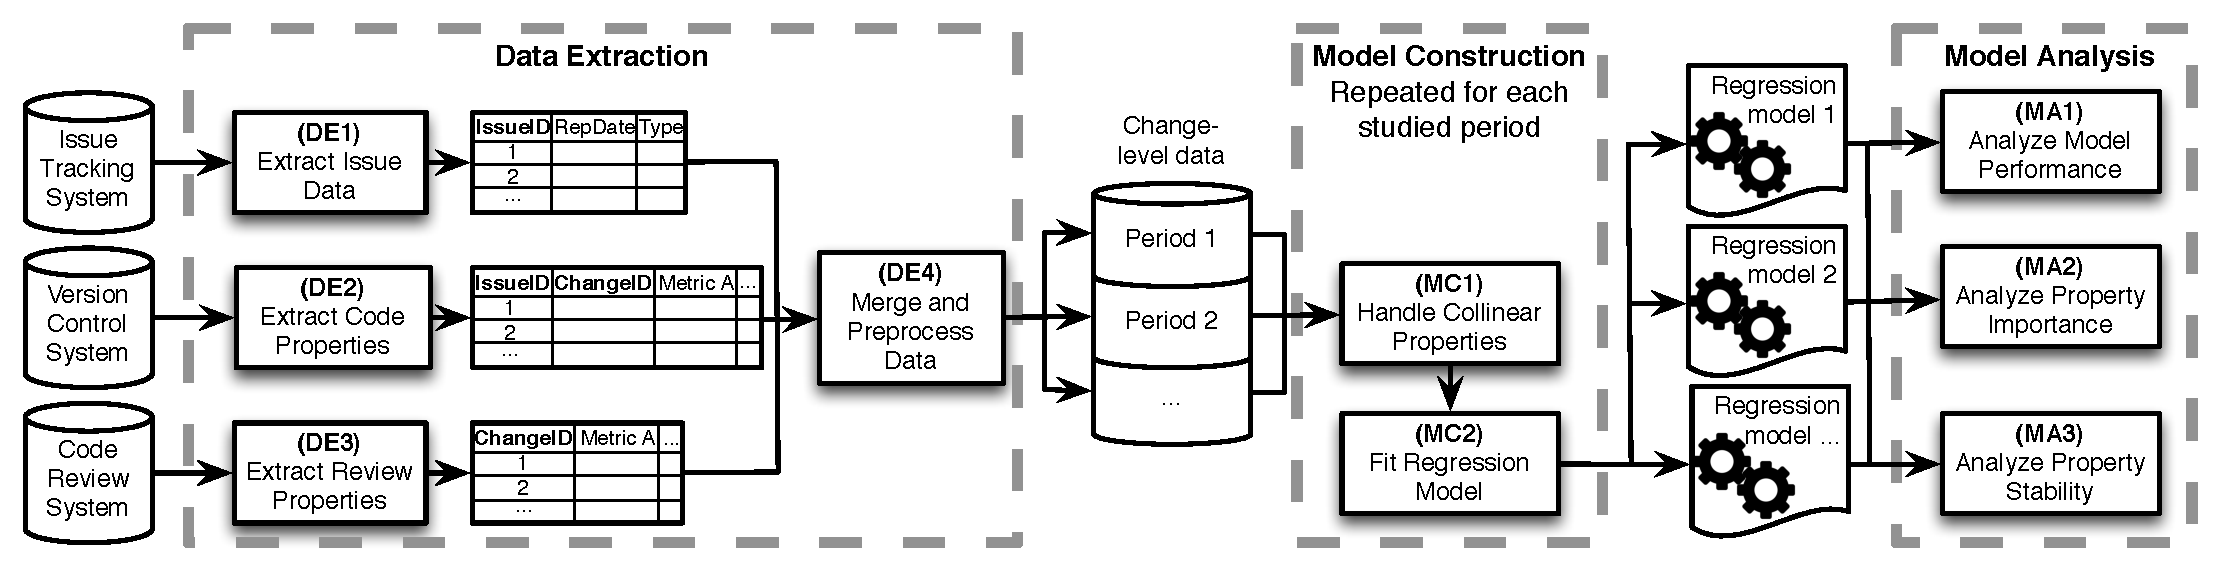
\includegraphics[width=0.98\textwidth]{figures/study_design.pdf}
\caption{An overview of the design of our case study.}
\label{fig:design}
\end{figure*}

\begin{table*}[ht!]
\centering
\caption{A taxonomy of the studied families of code and review properties.}
\label{tab:metrics}
\resizebox{\textwidth}{!}{
\begin{tabular}{c|p{2cm}|p{5.7cm}|p{8.4cm}}
\hline
& {\bf Property} & {\bf Description} & {\bf Rationale} \\
\hline
\multirow{2}{*}{\rotatebox{90}{Size}}
& Lines added & The number of lines added by a change. &  The more code that is changed, the more likely that defects \\
\cline{2-3}
& Lines deleted & The number of lines deleted by a change. & will be introduced~\cite{nagappan2006icse}.\\
\hline
\multirow{4}{*}{\rotatebox{90}{Diffusion}}
& Subsystems & The number of modified subsystems. & Scattered changes are riskier than focused ones because they \\
\cline{2-3}
& Directories & The number of modified directories. & require a broader spectrum of expertise~\cite{d2010extensive, hassan2009icse}.\\
\cline{2-3}
& Files & The number of modified files. &  \\
\cline{2-3}
& Entropy & The spread of modified lines across file. &  \\
\hline
\multirow{6}{*}{\rotatebox{90}{History}}
& Unique changes & The number of prior changes to the modified files. & More changes are likely more risky because developers will have to recall and track many previous changes~\cite{kamei2013tse}.\\
\cline{2-4}
& Developers & The number of developers who have changed the modified files in the past. & Files previously touched by more developers are likely more risky~\cite{matsumoto2010promise}. \\
\cline{2-4}
& Age & The time interval between the last and current changes. & More recently changed code is riskier than older code~\cite{graves2000tse}. \\
\hline
\multirow{11}{*}{\rotatebox{90}{Author/Rev. Experience}}
& Prior changes & The number of prior changes that an actor\smallnum{1} has participated in.\smallnum{2} & Changes that are produced by novices are likely to be more risky than changes produced by experienced developers~\cite{mockus2000bell}. \\
\cline{2-3}
& Recent changes & The number of prior changes that an actor has participated in weighted by the age of the changes (older changes are given less weight than recent ones). & \\
\cline{2-3}
& Subsystem changes & The number of prior changes to the modified subsystem(s) that an actor has participated in. & \\
\cline{2-4}
& Awareness\smallnum{3} & The proportion of the prior changes to the modified subsystem(s) that an actor has participated in. & Changes that involve developers who are aware of the prior changes in the impacted subsystems are likely to be less risky than those that do not. \\
\hline
\multirow{12}{*}{\rotatebox{90}{Review}}
& Iterations & Number of times that a change was revised prior to integration. & The quality of a change likely improves with each iteration. Hence, changes that undergo plenty of iterations prior to integration may be less risky than those that undergo few~\cite{porter1998tosem, thongtanunam2015msr}.\\
\cline{2-4}
& Reviewers & Number of reviewers who have voted on whether a change should be integrated or abandoned. & Since more reviewers will likely raise more issues so that they may be addressed prior to integration, changes with many reviewers are likely to be less risky than those with fewer reviewers~\cite{raymond}. \\
\cline{2-4}
& Comments & The number of non-automated, non-owner comments posted during the review of a change. & Changes with short discussions may not be deriving value from the review process, and hence may be more risky~\cite{mcintosh2014msr, mcintosh2016emse}.\\
\cline{2-4}
& Review window & The length of time between the creation of a review request and its final approval for integration. & Changes with shorter review windows may not have spent enough time carefully analyzing the implications of a change prior to integration, and hence may be more risky~\cite{porter1998tosem, thongtanunam2015msr}.\\
\hline
\multicolumn{4}{l}{\smallnum{1} Either the author or reviewer of a change. \smallnum{2} Either authored or reviewed. \smallnum{3} New property proposed in this paper.}
\end{tabular}
}
\end{table*}


\subsection{Data Extraction}

In order to conduct our case study, we extract data from the VCS, ITS, and code review databases of the studied systems.
Figure~\ref{fig:design} provides an overview of our data extraction approach.
Below, we describe each step in our approach.

\subsubsection*{(DE1) Extract Issue Data}
From each issue in the ITSs of the studied systems, we extract its unique identifier (IssueID), the timestamp from when the issue was reported (RepDate), and the issue type (Type, e.g., bug or enhancement).
The IssueID is used to link issues to code changes, while RepDate and Type are used to detect false positive links in our datasets.

\subsubsection*{(DE2) Extract Code Properties}
When extracting data from the VCS, we have three goals.
First, we detect whether a change is potentially fix-inducing or not using the SZZ algorithm~\cite{sliwerski2005msr}.
The SZZ algorithm identifies fix-inducing changes by:
(a) identifying defect-fixing changes,
(b) pinpointing the lines that are modified by defect-fixing changes using the {\tt diff} command,
and (c) traversing the version history to detect which change(s) introduced the modified lines using the {\tt blame} command.

Our second goal is to extract the IssueIDs and ChangeIDs that are encoded in commit messages.
The IssueIDs are used to link code changes to issue reports in the ITS, while the extracted ChangeIDs are used to link code changes to review records in the code review database.
The merging and preprocessing steps are defined in more detail under Step DE4 below.

Our third goal is to compute, for each change, four families of code change properties that have been shown to share a relationship with the likelihood of inducing fixes in past work~\cite{mockus2000bell, kim2008tse, kamei2013tse, kamei2016emse}.
We compute a broad range of code change properties that measure the change volume (Size), its dispersion across the codebase (Diffusion), the modified areas of the codebase (History), and the experience of the author (Author experience).
Table~\ref{tab:metrics} provides an overview of the studied properties.
We describe each family below.

\underline{\bf Size properties} measure the volume of code that was modified within the change.
For each change, we compute the number of {\em lines added} and {\em lines deleted}.
These properties can be directly computed by analyzing the change itself.

\newpage
\underline{\bf Diffusion properties} measure the dispersion of a change across a codebase.
For each change, we compute the number of distinct names of modified: (1) {\em subsystems} (i.e., root directories), (2) directories (i.e., full directories within the codebase), and (3) files.
To illustrate, consider the file {\tt qtbase/src/dbus/qdbuserror.cpp}.
The subsystem of this file is {\tt qtbase} and the directory is {\tt qtbase/src/dbus}.

\underline{\bf History properties} measure the past tendencies of modules that were involved with a change.
For each change, we measure history properties using the changes that have:
(a) modified the same files that are being modified by the change in question and
(b) been recorded prior to the change in question.
With this in mind, we compute the number of {\em unique changes} that have impacted the modified files in the past and the number of {\em developers} who have changed the modified files in the past.
We also compute the {\em age}, which is the average of the time intervals between the last change that was made to each modified file and the change in question.
Similar to prior studies~\cite{mockus2000bell, kamei2013tse}, we compute these history properties using all of the changes that were recorded prior to the change in question.

Files may be copied or renamed, which, if not handled carefully, may have an impact on our history properties.
In this paper, we rely on the built-in capability of {\tt git} to detect copied and renamed files.
When a copied/renamed file is detected, we include the history of the source of the copy/rename operation in the analysis of the target file.
Since {\tt git} copy/rename detection is based on heuristics, the detection results are not without limitations.
We discuss the potential impact that false positives and negatives may have on our history properties in Section~\ref{sec:cthreats}.

\begin{figure*}[t]
  \centering
  \subfloat[{\sc Qt}]{%
    \includegraphics[width=\columnwidth]{figures/filtering/qt_4.pdf}
    \label{fig:qt_filtering}
  }
  \subfloat[{\sc OpenStack}]{%
    \includegraphics[width=\columnwidth]{figures/filtering/openstack_4.pdf}
    \label{fig:openstack_filtering}
  }
  \caption{The rate of changes that are fix-inducing and the review coverage rate in the studied systems. The shaded areas are filtered out of our analysis due to large fluctuations in review coverage or drops in the rate of fix-inducing changes.}
  \label{fig:filtering}
\end{figure*}

\underline{\bf Author experience properties} estimate the expertise of the author of a change.
Similar to the history properties, author experience properties are computed using past changes.
The {\em experience} computes the number of past changes that an author has made to the codebase.
{\em Recent experience} weighs the experience value of changes by their age.
Similar to recent work~\cite{kamei2013tse}, we compute recent experience by applying $\frac{1}{1+\textit{age}}$, where {\em age} is measured in years.
{\em Subsystem experience} is the number of past changes that an author has made to the subsystems that are being modified by the change in question.
Finally, we propose author {\em awareness}---a new expertise property that measures the proportion of past changes that were made to a subsystem that the author of the change in question has authored or reviewed.
Again, Section~\ref{sec:cthreats} discusses the impact that {\tt git}'s copy/rename detection may have on our author experience measurements.

\subsubsection*{(DE3) Extract Review Properties}
When extracting data from the review databases of our studied systems, we have two goals.
First, we need to extract the ChangeIDs that are encoded in the review records.
These IDs uniquely identify a review record, and can be used to link them with code changes in the VCSs.
Next, we compute, for each review record, two families of properties that have been shown to share a relationship with the likelihood of inducing a fix~\cite{kononenko2015icsme,thongtanunam2015msr}.
We compute code review properties that measure the experience of the reviewer(s) (Reviewer experience) and characteristics of the review process (Review).
Table~\ref{tab:metrics} provides an overview of the studied review properties.
We describe each family below.

\underline{\bf Reviewer experience properties} estimate the expertise of the reviewers of a change.
Again, {\em experience} computes the number of past changes that a reviewer has reviewed,
{\em recent experience} weighs experience by age, and {\em subsystem experience} focuses on the subset of past reviews that have changed the same subsystems as the change in question.
Finally, {\em awareness} is the proportion of past changes that were made to a subsystem that the reviewer has authored or reviewed.
Again, we refer readers to Section~\ref{sec:cthreats} for a discussion of the impact that our reliance on {\tt git}'s built-in copy/rename detection may be having on our reviewer experience measurements.

\underline{\bf Review properties} estimate the investment that developers have made in the code review process.
{\em Iterations} counts the number of times that a code change was updated prior to integration.
{\em Reviewers} counts the number of developers who approved a change for integration.
{\em Comments} counts the number of reviewer comments that appear in a review record.
{\em Review window} is the length of the time interval between when a review record was opened and when the changes were approved for integration.

\begin{table}
\centering
\caption{The number of fix-inducing changes that survive each step of our filtering process.}
\label{tab:filterings}
\resizebox{\columnwidth}{!}{%
\begin{tabular}{l|p{2.5cm}|rrr|rrr}
\hline
\# & Filter & \multicolumn{3}{c|}{\sc Qt} & \multicolumn{3}{c}{\sc OpenStack} \\
   & & Total & \% & $\Delta$ & Total & \% & $\Delta$ \\
\hline
$F_0$ & No filters & 5,495 & 17\% & - & 4,423 & 16\% & - \\
$F_1$ & Code comments & 5,407 & 17\% & 88 & 4,291 & 16\% & 132 \\ 
$F_2$ & Whitespace changes  & 5,133 & 16\% & 274 & 3,814 & 14\% & 477 \\
$F_3$ & Issue report date   & 4,158 & 13\% & 975 & 3,480 & 13\% & 334 \\
$F_4$ & Issue report type & 3,242 & 10\% & 916 & 3,480 & 13\% & 0 \\
$F_{5a}$ & Too much churn & 3,190 & 10\% & 52 & 3,474 & 13\% & 6 \\
$F_{5b}$ & Too many files & 3,162 & 10\% & 28 & 3,461 & 13\% & 13 \\
$F_{5c}$ & No lines added & 3,153 & 11\% & 9 & 3,450 & 14\% & 11 \\
$F_6$ & Period & 2,891 & 11\% & 262 & 2,788 & 23\% & 662 \\
$F_7$ & Suspicious fixes & 2,172 & 9\% & 719 & 1,830 & 15\% & 958 \\
$F_8$ & Suspicious inducing changes & 2,002 & 8\% & 170 & 1,616 & 13\% & 214 \\
\hline
\end{tabular}
}
\end{table}

%F_4
%[metrics_qt5]$ awk -F, '{print $2}' all.metrics.csv.csv | sort -u | wc -l
%   31932
% awk -F, '{print $2}' qt.metrics.csv | sort -u | wc -l
%     225 -2 => 32,155
%[metrics_openstack]$ awk -F, '{print $2}' all.metrics.csv.csv | sort -u | wc -l
%   25268
% awk -F, '{print $2}' openstack.metrics.csv | sort -u | wc -l
%    1589 -2 => 26,855

\begin{comment}
# Here is the good example of white space filtering works:
-    def update_health_monitor(self, context,
-                              old_health_monitor,
-                              health_monitor,
-                              pool_id):
+    def update_pool_health_monitor(self, context,
+                                   old_health_monitor,
+                                   health_monitor,
+                                   pool_id):
\end{comment}


\subsubsection*{(DE4) Merge and Preprocess Data}
\label{sec:cleaning}

After extracting data from the VCSs, ITSs, and review databases of the studied systems, we merge them using the extracted identifiers (ChangeIDs and IssueIDs).
This merging allows us to filter our data to mitigate false positives in our datasets.
Table~\ref{tab:filterings} shows the impact of applying each filter sequentially to our sets of fix-inducing changes.

First, as suggested by Kim \ea~\cite{kim2006ase}, we ignore potential fix-inducing changes that only update code comments ($F_1$) or whitespace ($F_2$). 
Next, we filter out potential fix-inducing changes that appear after the date that the implicated defect was reported ($F_3$)~\cite{sliwerski2005msr}.
Then, we focus on only those defect-fixing changes where the issue type in the ITS is {\tt bug} ($F_4$).

After merging the datasets and cleaning the fix-inducing changes, we preprocess our dataset to remove extremities.
We ignore large commits---those that change at least 10,000 lines ($F_{5a}$) or at least 100 files ($F_{5b}$)---because these commits are likely noise that is caused by routine maintenance (e.g., copyright updates).
We also ignore changes that do not add any new lines ($F_{5c}$), since due to a limitation in the SZZ approach, only commits that introduce new lines have the potential to be flagged as fix-inducing.

In order to study whether properties of fix-inducing changes are consistent, we stratify our data into time periods.
We analyze period lengths of three and six months, since we find that at least three months are needed for our studied systems to accrue a substantial amount of data (i.e., 1,721--2,984 changes in {\sc Qt} and 831--2,094 in {\sc OpenStack}), while still yielding enough time periods to study trends (at least 18 periods in {\sc Qt} and 16 periods in {\sc OpenStack}).
Although the primary goal of our paper is not to identify the optimal period length, we discuss the threat that our choice of period lengths imposes on our conclusions in Section~\ref{sec:cthreats}.

Figure~\ref{fig:filtering} shows the results of a preliminary analysis of the rates of (a) fix-inducing changes and (b) reviewed changes in each time period ($F_6$).
We consider the rate of fix-inducing changes to counteract a limitation in the SZZ algorithm. 
The SZZ algorithm identifies defect-fixing changes, then traverses the version history to detect which change(s) had introduced the lines that were modified by the fix using the {\tt blame} command.
The SZZ algorithm needs future data to detect whether a change is fix-inducing or not.
Hence, the later the period in the analyzed data, the lower the chances that a fix has been committed to address the problems in those commits.
We do not filter out periods using a threshold value for the rate of fix-inducing changes in a period, but instead remove the latest periods where we begin to see a steady drop in the rate by analyzing Figure~\ref{fig:filtering}.

We also consider the rate of reviewed changes, since one of our criteria to select our subject systems is code review policy. However, even if the {\sc Qt} and {\sc OpenStack} projects have satisfied this criterion overall, the early periods of these projects may not.
These early periods of adoption of code review are likely turbulent as changes are being made to development processes.
To prevent the turbulent initial adoption period from impacting our reviewing measurements, we filter out periods where the review rate is low. 
Similar to the rate of fix-inducing changes, we do not select a threshold value for the rate of reviewed changes, but instead analyze Figure~\ref{fig:filtering} in search of suspicious values.

Figure~\ref{fig:qt_filtering} shows that code review coverage was sporadic in the early periods of {\sc Qt} development (periods 1--5).
Furthermore, the rate of fix-inducing changes drops dramatically in the final two development periods on record (periods 17 and 18).
Since this will introduce an additional confounding factor in our analysis, we elect to filter those periods out of our {\sc Qt} dataset.
Similarly, since Figure~\ref{fig:openstack_filtering} shows that code review coverage was extremely low for the first six development periods of {\sc OpenStack} (periods 1--6), we opt to filter those periods out of our {\sc OpenStack} dataset.

Finally, our recent work proposes a framework for evaluating the results of SZZ-generated data~\cite{costa2017tse}.
We use the framework to highlight suspicious fixes ($F_7$), i.e., changes that fix more than the upper Median Absolute Deviation (MAD) of the number of fixed issues by a change for that project.
Similarly, we use the framework to highlight suspicious fix-inducing changes as well ($F_8$), i.e., changes that induce more than the upper MAD of the number of fixes that were induced by a change for that project.

\subsection{Model Construction}
\label{sec:mc}

In this step, we use the preprocessed data to construct our JIT models.
Figure~\ref{fig:design} provides an overview of our model construction approach.
We describe each step below.

\subsubsection*{(MC1) Handle Collinear Properties}
Collinear code change properties will interfere with each other, distorting the modelled relationship between them and the likelihood of introducing defects.
Thus, we remove collinear properties prior to constructing our JIT models.

\underline{\bf Correlation analysis}:
We first check for code change properties that are highly correlated with one another using Spearman rank correlation tests ($\rho$).
We choose a rank correlation instead of other types of correlation (e.g., Pearson) because rank correlation is resilient to data that is not normally distributed.
We use a variable clustering analysis to construct a hierarchical overview of the correlation among the properties~\cite{varclus}.
For sub-hierarchies of code change properties with correlation $|\rho| > 0.7$, we select only one property from the sub-hierarchy for inclusion in our models.

\underline{\bf Redundancy analysis}:
In order to detect redundant code change properties, we fit preliminary models that explain each property using the others.
We use the $R^2$ value of these models to measure how well each property is explained by the others.
We use the implementation of this approach provided by the {\tt redun} function in the {\tt rms} R package, which iteratively drops the property that is most well-explained by the other properties until either:
(1) no model achieves an $R^2 \ge 0.9$,
or (2) removing a property would make a previously dropped property no longer explainable, i.e., its preliminary model will no longer achieve an R$^2 \ge 0.9$.

\subsubsection*{(MC2) Fit Regression Model}
We use a nonlinear variant of multiple regression modelling to fit our JIT models, which relaxes the assumption of a linear relationship between the likelihood of introducing defects and our code change properties.
This relaxed fitting technique enables a more accurate fit of the data. 
We allocate a maximum of three degrees of freedom to each property (i.e., allowing the relationship to change directions once).
Moreover, we fit our curves with restricted cubic splines, which fit smooth transitions at the points where curves change in direction (due to the curling nature of cubic curves).
Finally, as suggested by Harrell Jr. \ea~\cite{budget1, budget2}, we ensure that we do not exceed a ratio of 15 events (i.e., fix-inducing changes) per degree of freedom spent, which mitigates the risk of {\em overfitting}, i.e., producing a model that is too specialized for the training dataset to apply to others. 

The nonlinear variant of multiple regression modelling is often used in modelling of software engineering phenomena~\cite{mcintosh2016emse,morales2015saner,zhou2011icse}, especially for understanding the relationship between software development practices and software quality.
However, using other techniques may lead to different conclusions.
We discuss this threat to validity in Section~\ref{sec:ithreats}.

\subsection{Model Analysis}
\label{sec:ma}

Next, we address our research questions by analyzing our JIT models.
Figure~\ref{fig:design} provides an overview of our model analysis approach.
We describe each step below.

\subsubsection*{(MA1) Analyze Model Performance}
To assess the accuracy of our JIT models, we compute threshold-independent measures of model performance.
We avoid threshold-dependent measures like precision and recall, which depend on arbitrarily thresholds and are sensitive to imbalanced data.

The Area Under the receiver operator characteristics Curve (AUC) is a measure of a model's {\em discriminatory power}, i.e., its ability to differentiate between fix-inducing and clean changes.
AUC is computed by measuring the area under the curve that plots the true positive rate against the false positive rate, while varying the threshold that is used to determine if a change is classified as fix-inducing or not.
Values of AUC range between 0 (worst discrimination), 0.5 (random guessing), and 1 (perfect discrimination).

In addition to being a measure of discriminatory power, the Brier score is also a measure of a model's {\em calibration}, i.e., its absolute predictive accuracy.
The Brier score is computed as $\textit{Brier} = \frac{1}{N}\sum_{i=1}^{N}(y_i - \hat{y_i})^2$, where $N$ is the total number of changes; $y_i=1$ if the $i^{\textit{th}}$ change is fix-inducing, $y_i=0$ otherwise; and $\hat{y_i}$ is the probability of the $i^{\textit{th}}$ change being fix-inducing according to the JIT model under analysis.
It is important to note that low Brier scores are desirable.
Indeed, $\textit{Brier} = 0$ indicates perfect calibration, while $\textit{Brier} = 1$ indicates the worst possible calibration.

\subsubsection*{(MA2) Analyze Property Importance}
We estimate the impact that each family of code change properties has on the explanatory power of our JIT models.
In addition to each family being composed of several properties, each property has been allocated several degrees of freedom due to our nonlinear model construction approach (see Section~\ref{sec:mc}).
Each degree of freedom is represented with a model term.
Hence, to control for the effect of multiple properties (and multiple terms), we jointly test the set of model terms for each family using Wald $\chi^2$ maximum likelihood (a.k.a., ``chunk'') tests~\cite{frank}.
In order to make the Wald $\chi^2$ values of multiple models comparable, we normalize them by the total Wald $\chi^2$ score of the JIT model from which they originate.
The larger the normalized Wald $\chi^2$ score, the larger the impact that a particular family of properties has on the explanatory power of the JIT model under analysis.

\subsubsection*{(MA3) Analyze Property Stability}
To assess the stability of the importance scores for a family of code change properties $f$ over time, we compute the difference between the importance scores of $f$ in a model that is trained using time period $p$ and a future model that is trained using time period $p+x$, where $x>0$.

\section{Case Study Results}
\label{sec:results}

In this section, we present the results of our case study with respect to our research questions.
For each research question, we present our approach and discuss the results.

\subsection*{(RQ1) \rqi}

\begin{figure}
  \centering
  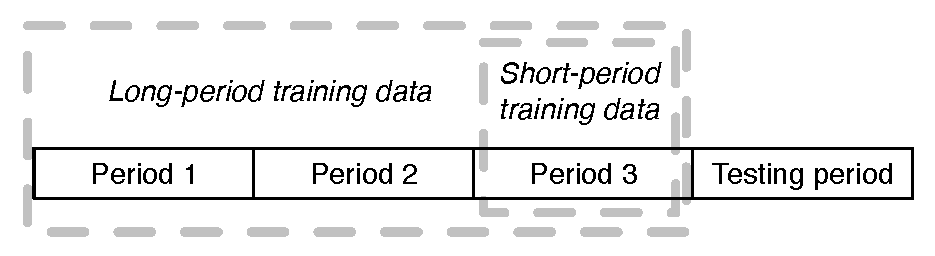
\includegraphics[width=0.9\columnwidth]{figures/period_examples.pdf}
  \caption{An illustrative example of the types of the JIT model types.}
  \label{fig:period_ex}
\end{figure}

\begin{figure*}[t]
  \centering
  \subfloat[AUC in three-month periods ({\sc Qt})]{
    \includegraphics[width=0.88\columnwidth]{figures/perf/qt_lrm_4_AUC.pdf}
    \label{fig:perf_qt_auc}
  }
  \subfloat[AUC in six-month periods ({\sc Qt})]{
    \includegraphics[width=0.88\columnwidth]{figures/perf/qt_lrm_2_AUC.pdf}
    \label{fig:six_perf_qt_auc}
  }
  \qquad
  \subfloat[AUC in three-month periods ({\sc OpenStack})]{
    \includegraphics[width=0.88\columnwidth]{figures/perf/openstack_lrm_4_AUC.pdf}
    \label{fig:perf_openstack_auc}
  }
  \subfloat[AUC in six-month periods ({\sc OpenStack})]{
    \includegraphics[width=0.88\columnwidth]{figures/perf/openstack_lrm_2_AUC.pdf}
    \label{fig:six_perf_openstack_auc}
  }
  \qquad
  \subfloat[Brier score in three-month periods ({\sc Qt})]{
    \includegraphics[width=0.88\columnwidth]{figures/perf/qt_lrm_4_Brier.pdf}
    \label{fig:perf_qt_brier}
  }
  \subfloat[Brier score in six-month periods ({\sc Qt})]{%
    \includegraphics[width=0.88\columnwidth]{figures/perf/qt_lrm_2_Brier.pdf}
    \label{fig:six_perf_qt_brier}
  }
  \qquad
  \subfloat[Brier score in three-month periods ({\sc Openstack})]{
    \includegraphics[width=0.88\columnwidth]{figures/perf/openstack_lrm_4_Brier.pdf}
    \label{fig:perf_openstack_brier}
  }
  \subfloat[Brier score in six-month periods ({\sc OpenStack})]{%
    \includegraphics[width=0.88\columnwidth]{figures/perf/openstack_lrm_2_Brier.pdf}
    \label{fig:six_perf_openstack_brier}
  }
  \caption{The predictive performance of JIT models as the studied systems age.}
  \label{fig:perf}
\end{figure*}

\begin{figure*}[t]
  \centering
  \subfloat[AUC in three-month periods ({\sc Qt})]{
    \includegraphics[width=0.88\columnwidth]{figures/perf/qt_lrm_4_AUC_delta.pdf}
    \label{fig:perf_qt_auc_delta}
  }
  \subfloat[AUC in six-month periods ({\sc Qt})]{
    \includegraphics[width=0.88\columnwidth]{figures/perf/qt_lrm_2_AUC_delta.pdf}
    \label{fig:six_perf_qt_auc_delta}
  }
  \qquad
  \subfloat[AUC in three-month periods ({\sc OpenStack})]{%
    \includegraphics[width=0.88\columnwidth]{figures/perf/openstack_lrm_4_AUC_delta.pdf}
    \label{fig:perf_openstack_auc_delta}
  }
  \subfloat[AUC in six-month periods ({\sc OpenStack})]{%
    \includegraphics[width=0.88\columnwidth]{figures/perf/openstack_lrm_2_AUC_delta.pdf}
    \label{fig:six_perf_openstack_auc_delta}
  }
  \qquad
  \subfloat[Brier score in three-month periods ({\sc Qt})]{
    \includegraphics[width=0.88\columnwidth]{figures/perf/qt_lrm_4_Brier_delta.pdf}
    \label{fig:perf_qt_brier_delta}
  }
  \subfloat[Brier score in six-month periods ({\sc Qt})]{
    \includegraphics[width=0.88\columnwidth]{figures/perf/qt_lrm_2_Brier_delta.pdf}
    \label{fig:six_perf_qt_brier_delta}
  }
  \qquad
  \subfloat[Brier score in three-month periods ({\sc OpenStack})]{%
    \includegraphics[width=0.88\columnwidth]{figures/perf/openstack_lrm_4_Brier_delta.pdf}
    \label{fig:perf_openstack_brier_delta}
  }
  \subfloat[Brier score in six-month periods ({\sc OpenStack})]{%
    \includegraphics[width=0.88\columnwidth]{figures/perf/openstack_lrm_2_Brier_delta.pdf}
    \label{fig:six_perf_openstack_brier_delta}
  }
  \caption{The delta in the estimated performance of JIT models as the studied systems age.}
  \label{fig:perf_delta}
\end{figure*}

\smallsection{RQ1: Approach}
To address RQ1, we study how quickly a JIT model loses its predictive power by training JIT models for each of the time periods (i.e., varying the training period), and measuring their performance on future periods.
As illustrated in Figure~\ref{fig:period_ex}, for each period, we train two types of models:

\begin{enumerate}
  \item \underline{\bf Short-period models} are JIT models that are only trained using changes that occurred during one time period.
    We train short-period models because older changes may have characteristics that no longer apply to the latest changes.
  \item \underline{\bf Long-period models} are JIT models that are trained using all of the changes that occurred during or prior to a particular period.
    We train long-period models because recent work suggests that larger amounts of training data tend to yield defect models that perform better, even when biases are introduced~\cite{rahman2013fse}.
    Hence, despite potential changes in the properties of fix-inducing changes, being exposed to additional data may improve the performance of our JIT models.
\end{enumerate}

After training our JIT models, we test their performance when they are applied to the periods that occur after the last training period.
As described in Section~\ref{sec:ma}, we measure the performance of our models using the AUC (discriminatory power) and the Brier score (calibration).

For example, Figure~\ref{fig:period_ex} illustrates that for a training period 3, the short-period model is trained using the changes that occurred during period 3, while the long-period model is trained using changes that occurred during periods 1, 2, and 3.
These short-period and long-period models of period 3 are tested using periods 4 through to the last studied period.
The AUC and Brier performance scores are computed for each testing period individually.

Finally, we plot the trends in AUC and Brier performance scores over time using heatmaps.
In Figure~\ref{fig:perf}, the shade of a box indicates the performance value, where blue shades indicate strong performance, red shades indicate weak performance, and the palest (white) shade indicates the performance that a random guessing model would achieve (on average).
In Figure~\ref{fig:perf_delta}, the shade indicates the difference in AUC and Brier performance scores between the training and testing periods in question.
Red, blue, and pale (white) shades indicate drops, improvements, and unchanged performance in the testing period, respectively.

\smallsection{RQ1: Results}
\textbf{Models that are trained using periods that are closer to the testing period tend to outperform models that are trained using older periods.}
When we focus on the columns of Figure~\ref{fig:perf}, the performance values tend to improve as the training period increases.
In {\sc Qt}, the trend is especially prominent in testing periods 5 and later of the three-month period models, where at least one year has elapsed.
For example, the long-period sections of Figures~\ref{fig:perf_qt_auc} and~\ref{fig:perf_openstack_auc} show an AUC score improvement of 16--24 percentage points for {\sc Qt} and 6--12 percentage points for {\sc OpenStack} by training using the most recent data (i.e., the period just prior to the testing period) instead of the data from period 1.
Figures~\ref{fig:perf_qt_brier} and~\ref{fig:perf_openstack_brier} also show a boost in Brier score of 12--28 and 6--7 percentage points for {\sc Qt} and {\sc OpenStack}, respectively.

Although the magnitude is lower, similar improvement trends are observed in the six-month periods.
Figures~\ref{fig:six_perf_qt_auc} and~\ref{fig:six_perf_openstack_auc} show an AUC score improvement of 5--6 percentage points in {\sc Qt} and 9 percentage points in {\sc OpenStack}.
While Figure~\ref{fig:perf_qt_brier} shows an improvement in Brier score of only 1 percentage point for {\sc Qt}, Figure~\ref{fig:perf_openstack_brier} shows a boost of 5 percentage points for {\sc OpenStack}.

The improving trend tends to stabilize (at least) one period before the testing period.
For example, Figures~\ref{fig:perf_qt_auc} and~\ref{fig:perf_openstack_auc} show that the AUC improvement gained by adding the most recent three-month period to the long-period models of both studied systems is -1--2 percentage points.
The -1 indicates a 1 percentage point loss in testing periods 6 and 8 of {\sc Qt} (0.68 and 0.67 in training periods 4 and 5) and {\sc OpenStack} (0.64 and 0.63 in training periods 5 and 6), respectively.
Figures~\ref{fig:six_perf_qt_auc} and~\ref{fig:six_perf_openstack_auc} show similar trends of adding the most recent six-month period to the long-period models of both studied systems yields improvements of 0--3 percentage points.
Figures~\ref{fig:perf_qt_brier},~\ref{fig:six_perf_qt_brier},~\ref{fig:perf_openstack_brier}, and~\ref{fig:six_perf_openstack_brier} show similar fluctuations of 0--2 percentage points in Brier score.

\textbf{Our models lose a large amount of predictive power one year after being trained.}
Analysis of the rows of Figure~\ref{fig:perf_delta} shows that after one year, there is often a large drop in the AUC and a sharp increase in the Brier score.
Figures~\ref{fig:perf_qt_auc_delta} and~\ref{fig:perf_openstack_auc_delta} show that our short-period models lose 3--22 and 3--34 AUC percentage points one year after being trained (i.e., $\textit{testing period} = \textit{training period} + 4$) in {\sc Qt} and {\sc OpenStack}, respectively.
The drops of only three AUC percentage points are observed in period 7 of {\sc Qt} and period 9 of {\sc OpenStack}, which Figures~\ref{fig:perf_qt_auc} and~\ref{fig:perf_openstack_auc} show have a tendency to yield strong performance scores (with performance scores noticeably higher than those of nearby rows).
If those periods are omitted, the drops in AUC associated with our short-period models range from 11--22 percentage points in {\sc Qt} and 14--34 percentage points in {\sc OpenStack}.
Moreover, while training periods 1 and 2 of the long-period models in {\sc Qt} also suffer from large AUC drops of 22 and 13 percentage points, respectively, our long-period models that we train using periods 5 and later tend to retain their predictive power, only losing 1--9 AUC percentage points after one year.
Similarly, after one year, the Brier score of our {\sc Qt} and {\sc OpenStack} models drop by up to 11 and 19 percentage points, respectively (see Figures~\ref{fig:perf_qt_brier_delta} and \ref{fig:perf_openstack_brier_delta}).


Interestingly, Figures~\ref{fig:perf_qt_auc_delta},~\ref{fig:six_perf_qt_auc_delta},~\ref{fig:perf_qt_brier_delta}, and~\ref{fig:six_perf_openstack_brier_delta} show that after losing a large amount of predictive power after one year, our {\sc Qt} and {\sc OpenStack} models of periods 1 and 2 recover some predictive power in later periods.
This suggests that the properties of fix-inducing changes in those later periods share some similarities with the fix-inducing changes of the earliest periods.
We investigate this in RQ2.

\textbf{Long-period JIT models do not always retain predictive power for longer than short-period JIT models.}
Note that the short-period and long-period models for period 1 are identical because there is no additional data added when training the long-period model.
Hence, we only discuss the improvement in retention of predictive power for the JIT models that are trained using periods 2 and later.

We observe improvements in the predictive power of our {\sc Qt} models when they are tested in both the three-month and six-month settings.
The rows of Figures~\ref{fig:perf_qt_auc_delta} and~\ref{fig:six_perf_qt_auc_delta} show that the long-period models of periods 2 and later retain more predictive power than their short-period counterparts in terms of AUC.
For example, Figure~\ref{fig:perf_qt_auc_delta} shows that the short-period model that was trained using period 3 drops 8 percentage points in AUC when it is tested on period 4, while the long-period model only drops 5 percentage points under the same circumstances.
Moreover, Figure~\ref{fig:six_perf_qt_auc_delta} shows that long-period models in the six-month period setting drop at most 3 percentage points of AUC when they are tested on the final period (period 6), while short-period models drop up to 10 percentage points.
Figures~\ref{fig:perf_qt_brier_delta} and~\ref{fig:six_perf_qt_brier_delta} show that there is also an improvement in the retention of Brier score for {\sc Qt}.

Surprisingly, in {\sc OpenStack}, Figures~\ref{fig:perf_openstack_auc_delta} and~\ref{fig:perf_openstack_brier_delta} show
 that the long-period models underperform with respect to the short-period models in terms of AUC and Brier score.
 This suggests that fix-inducing changes vary from period to period, with a sensitivity to more recent changes being more beneficial than accruing additional data in {\sc OpenStack}.

\conclusionbox{A large proportion of the predictive power of JIT models is lost one year after being trained, suggesting that properties of fix-inducing changes may be in flux. JIT performance decay can be dampened by training JIT models using data that is recorded nearer to the testing period (i.e., more recent data).}

\subsection*{(RQ2) \rqii}

\smallsection{RQ2: Approach}
In order to address RQ2, we compute the normalized Wald $\chi^2$ importance scores (see Section~\ref{sec:ma}) of each studied family of code change properties in each of our short-period and long-period JIT models.
We study trends in the importance scores using heatmaps.
The darker the shade of a given box, the more important that that family is to our model fit for that period.
Figure~\ref{fig:importance} shows the results of our family importance analysis.
In addition, we compute the p-values that are associated with the importance scores and denote the significance of each cell using asterisks (*).

\smallsection{RQ2: Results}
\textbf{The Size family is a consistent top-contributor to the fits of our models.}
Figure~\ref{fig:importance} shows that Size is often the most darkly shaded cell per period (columns).
Figures~\ref{fig:importance_qt} and~\ref{fig:six_importance_qt} show that in {\sc Qt}, the Size family accounts for 23\%--38\% and 23\%--37\% of the explanatory power of our three- and six-month long-period JIT models, respectively.
Moreover, Size accounts for 10\%--43\% and 13\%--37\% of the explanatory power of our three- and six-month short-period JIT models, respectively.
Figures~\ref{fig:importance_qt} and~\ref{fig:six_importance_qt} also show that the Size family is the top contributor in 8 of the 11 three-month periods and 5 of the 6 six-month periods of our short-period JIT models, and all of the three- and six-month periods for our long-period JIT models.
The contributed explanatory power of the Size family is statistically significant in all of the periods for our short- and long-period models in both three- and six-month settings ($p < 0.05$ and $p < 0.01$, respectively).

Similarly, Figures~\ref{fig:importance_openstack} and~\ref{fig:six_importance_openstack} show that in {\sc OpenStack}, the Size family accounts for 11\%--37\% and 15\%--19\% of the explanatory power of our three- and six-month long-period JIT models, respectively. 
Size also contributes 3\%--37\% and 14\%--25\% of the explanatory power of our three- and six-month short-period JIT models, respectively.
Moreover, Size is only a non-significant contributor to two of the nine three-month short-period models, providing a significant amount of explanatory power to all of the other three-month short- and long-period models, as well as all of the six-month short- and long-period models.
In short, the magnitude and consistency of the importance of Size suggests that advice about limiting change size is sound.

\begin{figure*}[t]
  \centering
  \subfloat[Three-month periods ({\sc Qt})]{
    \includegraphics[width=0.95\columnwidth]{figures/importance/qt_lrm_4.pdf}
    \label{fig:importance_qt}
  }
  \subfloat[Six-month periods ({\sc Qt})]{
    \includegraphics[width=0.95\columnwidth]{figures/importance/qt_lrm_2.pdf}
    \label{fig:six_importance_qt}
  }
  \qquad
  \subfloat[Three-month periods ({\sc OpenStack})]{%
    \includegraphics[width=0.95\columnwidth]{figures/importance/openstack_lrm_4.pdf}
    \label{fig:importance_openstack}
  }
  \subfloat[Six-month periods ({\sc OpenStack})]{%
    \includegraphics[width=0.95\columnwidth]{figures/importance/openstack_lrm_2.pdf}
    \label{fig:six_importance_openstack}
  }
  \caption{How the importance scores of the studied families of code change properties change over time. Shade indicates magnitude while asterisks indicate significance according to Wald $\chi^2$ test, where: * $p < 0.05$; ** $p < 0.01$; *** $p < 0.001$.}
  \label{fig:importance}
\end{figure*}

While the explanatory power of the Size family often dominates our models, there are periods where other families have larger importance scores.
For example, Figures~\ref{fig:importance_openstack} and~\ref{fig:six_importance_openstack} also show that in {\sc OpenStack}, the Review family achieves a larger importance score than the Size family in:
(a) periods 2, 3, and 6 of the three-month short-term models,
(b) periods 2--7 of the three-month long-period models,
(c) periods 1--3 of the six-month short-term models,
and (d) all periods of the six-month long-term models.
Figures~\ref{fig:importance_qt} shows that in {\sc Qt}, the Review family achieves a larger importance score than the Size family in periods 5, 6, and 9 of the three-month short-term models, while the History family achieves a larger importance score than the Size family in the short-period model of period 6.

\textbf{Fluctuations in family importance are common in short-period models.}
Figure~\ref{fig:importance} shows that the shades of family importance (rows) vary more in short-period models than they do in long-period models.
For example, in the three-month periods of {\sc Qt} (Figure~\ref{fig:importance_qt}), the delta of the maximum and minimum explanatory power in the Size family is 0.33 ($0.43 - 0.10$) and 0.15 ($0.38 - 0.23$) in the short- and long-period settings, respectively.
This is as one might expect, given that long-period models are eventually trained using much more data.
Nonetheless, varying family importance in short-period models is another indication of fluctuation of the properties of fix-inducing changes.

Fluctuations in family importance also do occur in long-period models, albeit less often than short-period models.
For example, Figure~\ref{fig:importance_openstack} shows that Diffusion, Reviewer Experience, and Review importance scores grow and shrink over the studied periods.
Reviewer Experience increases and decreases in importance as {\sc OpenStack} ages, while the importance of the Reviewer Experience and Diffusion fades in the early periods and grows again in later periods.

\textbf{Our awareness measures do not contribute a significant amount of explanatory power.}
In this paper, we propose author and reviewer awareness---two new code change properties that compute how much of the prior change activity the author and reviewer has been involved with (see Table~\ref{tab:metrics}).
Analysis of our model fits reveals that the awareness change properties did not improve our fits to a statistically significant degree.
In fact, author awareness is often highly correlated with other Experience properties, suggesting that in the studied systems, author awareness does not provide any new information that existing Experience measures do not already capture.
Despite the negative outcome of this empirical analysis, it may still be worthwhile to compute awareness values in future studies, since larger amounts of data may provide an opportunity for awareness values to differ from those of other Experience measures.

\conclusionbox{The importance of most families of code change properties fluctuate from period to period, suggesting that the properties of fix-inducing changes tend to evolve as projects age.}

\subsection*{(RQ3) \rqiii}

\begin{figure*}[t]
  \centering
  \subfloat[Three-month periods ({\sc Qt})]{
    \includegraphics[width=0.7\textwidth]{figures/stability/qt_lrm_4.pdf}
    \label{fig:stability_qt}
  }
  \subfloat[Six-month periods ({\sc Qt})]{
    \includegraphics[width=0.3\textwidth]{figures/stability/qt_lrm_2.pdf}
    \label{fig:six_stability_qt}
  }
  \vspace{-2mm}
  \qquad
  \subfloat[Three-month periods ({\sc OpenStack})]{%
    \includegraphics[width=0.7\textwidth]{figures/stability/openstack_lrm_4.pdf}
    \label{fig:stability_openstack}
  }
  \subfloat[Six-month periods ({\sc OpenStack})]{%
    \includegraphics[width=0.3\textwidth]{figures/stability/openstack_lrm_2.pdf}
    \label{fig:six_stability_openstack}
  }
  \caption{The stability of the importance scores of the studied families of code change properties over time ($\textit{FISDiff}(f,i,j)$).}
  \label{fig:stability}
\end{figure*}

\smallsection{RQ3: Approach}
To address RQ3, we study the stability of the importance scores of the studied families of code change properties.
To do so, we first select the short-period and long-period JIT models that we trained using each of the time periods.
For each model, we compute the Family Importance Score ($\textit{FIS}$) for each family $f$ in:
(a) the training period $i$ ($\textit{FIS}(f,i)$) and
(b) the short-period JIT models in each period $j$ in the year that follows after the training period (i.e., $\textit{FIS}(f,j)$, where $j \in \{i+1, i+2, \cdots, i+\textit{\# periods per year}\}$)).
The $\textit{FIS}(f,n)$ is the jointly tested model terms for all of the metrics belonging to a family $f$ in the model of period $n$.
Note that when computing $\textit{FIS}(f,j)$ (i.e., those values that belong to ``future'' time periods), we use short-period JIT models instead of long-period models because short-period models should more accurately reflect the characteristics of the period in question.
We then compute the differences between the importance scores in periods $i$ and $j$ using $\textit{FISDiff}(f,i,j) = \textit{FIS}(f,i) - \textit{FIS}(f,j)$.

It is important to note that $\textit{FISDiff}(f,i,j) > 0$ indicates that the importance of family $f$ is larger in period $i$ (the training period) than it is in period $j$, i.e., the JIT model that is trained using period $i$ {\em overestimates} the future importance of family $f$.
In these situations, quality improvement plans that are based on the importance of $f$ at the end of period $i$ would have a smaller impact than anticipated.

On the other hand, $\textit{FISDiff}(f,i,j) < 0$ indicates that the importance of family $f$ is smaller in period $i$ than it is in period $j$, i.e., the JIT model that is trained using period $i$ {\em underestimates} the importance of family $f$.
In these situations, quality improvement plans that are based on the importance of $f$ in period $i$ may miss important families that would yield larger quality improvements than anticipated.

Similar to RQ2, we show the $\textit{FISDiff}(f,i,j)$ values using heatmaps.
We also compute the p-values that are associated with the importance score of the model of period $i$, since this is the model upon which quality improvement plans would be based.
We again denote the statistical significance of these importance scores using asterisks (*).
For presentation clarity, we only show $\textit{FISDiff}(f,i,j)$ values for the year that follows the training of each model.
As shown below, this one-year period is enough to demonstrate interesting trends.

\smallsection{RQ3: Results}
{\textbf{Long-period models should be preferred for quality improvement planning.}
The short-period models of Figure~\ref{fig:importance} show several periods where trends in importance fluctuate sporadically.
These spikes and troughs in importance scores can have a misleading impact on quality improvement plans when they are the source of data that is used to train JIT models.
Figure~\ref{fig:stability} shows that long-period models tend to cope with these periods of sporadic fluctuation more gracefully than short-period models do.

For example, Figure~\ref{fig:importance_qt} shows that the Size family has a large spike in importance in period 7 of the three-month setting of {\sc Qt}.
Training periods 5 and 6 of Figure~\ref{fig:stability_qt} show that the importance of the Size family is underestimated by 18 and 22 percentage points, respectively for testing period 7 in short-period models.
Since the long-period models have a smoothing effect, these underestimates drop to 7 and 9 percentage points, respectively.
When period 7 becomes the training period in Figure~\ref{fig:stability_qt}, the impact of the Size family is overestimated by up to 23 percentage points in the short-period models.
The maximum overestimate for the related long-period models is 15 percentage points.

Turning to {\sc OpenStack}, Figure~\ref{fig:importance_openstack} shows that the Review family has a large spike in importance in period 6.
Training periods 4 and 5 of Figure~\ref{fig:stability_openstack} show that the importance of the Review family is underestimated by 57 and 46 percentage points, respectively in the short-period models.
Again, the smoothing effect of the long-period reduces the impact of this spike to 27 and 29 percentage points, respectively.

The six-month setting (Figures~\ref{fig:six_stability_qt} and~\ref{fig:six_stability_openstack}) shows less severe over/underestimates, also suggesting that larger amounts of training data will smooth the impact of period-specific fluctuations on quality improvement plans.

\textbf{The stability of many families of code change properties is project-sensitive.}
For example, the consistency of blue-shaded cells in Figure~\ref{fig:stability_qt} indicates that the importance of the Size family is often overestimated in {\sc Qt} (median of 5\%), especially in training period 2.
Indeed, Figure~\ref{fig:importance_qt} shows that importance of Size was largest at training period 2 of {\sc Qt}, trending downwards after that.
Conversely, the consistency of red-shaded cells in Figure~\ref{fig:stability_openstack} indicates that the importance of the Size family is often underestimated in {\sc OpenStack} (median of 2\%), especially in training periods 2 and 3.
Again, Figure~\ref{fig:importance_openstack} shows that importance of Size is growing as {\sc OpenStack} ages from period 2 and 3.
Models that are trained using the early periods tend to underestimate the importance of the Size family in later periods.

Similarly, Figure~\ref{fig:stability_qt} shows that the History family tends to be underestimated in {\sc Qt} (13 out of 24 periods for short-period and 20 out of 24 periods for long-period), while Figure~\ref{fig:stability_openstack} shows that the Review family tends to be overvalued in {\sc OpenStack} (17 out of 20 periods for short-period and 19 out of 20 periods for long-period).
Indeed, Figure~\ref{fig:importance_qt} shows that the History family tends to grow more important as {\sc Qt} ages, while Figure~\ref{fig:importance_openstack} shows that the Review family tends to become less important as {\sc OpenStack} ages.

%\todo{Diffusion, Rev. Exp, Review are not discussed.}

\conclusionbox{When constructing quality improvement plans, one should favour large caches of data (e.g., long-period models, six-month periods).
The importance of impactful families of code change properties like Size and Review are consistently under/overestimated in the studied systems.}

\section{Practical Suggestions}
\label{sec:practice}

Based on our findings, we make the following suggestions for practitioners:

\begin{enumerate}[{\bf (1)}]
  \item {\bf JIT models should be retrained to include data from at most three months prior to the testing period.}
    Our findings from RQ1 suggest that JIT models lose a large amount of predictive power one year after they are trained using the datasets that are collected from early periods.
    To avoid producing misleading predictions, JIT models should be retrained using more recent data often, at least more than once per year.

 

  \item {\bf Long-term JIT models should be trained using a cache of plenty of changes.}
    Complementing recent work on module-level defect predictors~\cite{rahman2013fse}, our findings from RQ1 indicate that larger amounts of data (i.e., our long-period models) can dampen performance decay in JIT models.
    Indeed, JIT models that are trained using more changes tend to retain their predictive power for a longer time than JIT models that are trained only using the changes that were recorded during most recent three-month period.

  \item {\bf Quality improvement plans should be revisited periodically using feedback from recent data.}
    Our findings from RQ2 suggest that the importance of code change properties fluctuates over time.
    Moreover, our findings from RQ3 suggest that these fluctuations can lead to misalignments of quality improvement plans.
    Since RQ3 shows that long-period models achieve better stability, they should be preferred when making short-term quality plans.
    For long-term plans, we note that families for whom their importance scores were underestimated (overestimated) in the past tend to also be underestimated (overestimated) in the future.
    Hence, quality improvement plans should be periodically reformulated using the stability of the importance scores in the past to amplify or dampen raw importance scores.
\end{enumerate}

\section{Threats to Validity}
\label{sec:threats}

We now discuss the threats to the validity of our study.

\subsection{Construct Validity}
\label{sec:cthreats}

Threats to construct validity have to do the alignment of our choice of indicators with what we set out to measure.
We identify fix-inducing changes in our datasets using the SZZ algorithm~\cite{sliwerski2005msr}.
The SZZ algorithm is commonly used in defect prediction research~\cite{kim2008tse, kamei2013tse, kamei2016emse, kononenko2015icsme}, yet has known limitations.
For example, if a defect identifier is not recorded in the VCS commit message of a change, it will not be flagged as defect-fixing.
To combat this potential bias, we select systems that use the Gerrit code reviewing tool, which tightly integrates with the VCS, allowing projects to automatically generate reliable commit messages based on fields of the approved code reviews.
These commit messages can easily be processed.
Hence, insofar as developers are carefully filling in code review records in Gerrit, our VCS data will be clean.
Nonetheless, an approach to recover missing links that improves the accuracy of the SZZ algorithm~\cite{wu2011fse} may further improve the accuracy of our results.

Similarly, we conduct a preliminary analysis of the rates of
(a) fix-inducing changes and
(b) reviewed changes in each time period to mitigate limitations of the SZZ algorithm and to prevent the turbulent initial adoption periods from impacting our reviewing measurements.
Although the preliminary analysis is conducted to mitigate false positives in our datasets of fix-inducing changes, it may bias our results.

Copied and renamed files may truncate our history and experience code change properties.
We rely on the copied and renamed file detection algorithms that are built into the {\tt git} VCS.
Since these algorithms are based on heuristics, they may introduce false positives or false negatives.
To check how serious concerns of false positives are, we selected a sample of 50 files that were identified as copied/renamed from our dataset.
In our opinion, all of these files were indeed copied/renamed, suggesting that false positives are not severely affecting our measurements.
False negatives are more difficult to quantify.
Nonetheless, a more accurate copy/rename detection technique may yield more accurate history and experience measurements.

More broadly speaking, our code change measurements are computed using various scripts that we have written.
These scripts may themselves contain defects, which would affect our measurements and results.
We combat this threat by testing our tools and scripts on subsamples of our datasets, and manually verifying the results.

Our results may be sensitive to the period length.
We select period lengths of three and six months such that each period contains a sufficient amount of data to train stable defect models, while still yielding enough periods to study evolutionary trends.
Moreover, this paper aims to study changes in the properties of fix-inducing changes over time, not to identify the ``optimal'' period length.

\subsection{Internal Validity}
\label{sec:ithreats}

Threats to internal validity have to do with whether other plausible hypotheses could explain our results.
We assume that fluctuations in the performance and impactful properties of JIT models are linked with fluctuations in the nature of fix-inducing changes.
However, other intangible confounding factors could be at play (e.g., changes to team culture, contributor turnover).
On the other hand, we control for six families of code change properties that cover a broad range of change characteristics.

Our findings may be specific to nonlinear logistic regression models, and may not apply to other classification techniques.
As suggested by our prior work~\cite{ghotra2015icse}, we are actively investigating other classification techniques like Random Forest.
Preliminary results indicate that the findings of RQ1 can be reproduced in the Random Forest context.
However, since the Wald $\chi^2$ importance scores are not well-defined for such classifiers, a common importance score needs to be identified before RQ2 and RQ3 can be replicated.

\subsection{External Validity}

Threats to external validity have to do with the generalizability of our results to other systems.
We focus our study on two open source systems.
We chose strict eligibility criteria, which limits the systems that are available for analysis (see Section~\ref{sec:studied}).
Due to our small sample size, our results may not generalize to all software systems.
However, the goal of this paper is not to build a grand theory that applies to all systems, but rather to show that there are some systems for which properties of fix-inducing changes are fluctuating.
Our results suggest that these fluctuations can have a large impact on the performance of JIT models and the quality improvement plans that are derived from JIT models.
Nonetheless, additional replication studies are needed to generalize our results.

\section{Conclusions \& Future Work}
\label{sec:conclusions}

JIT models are trained to identify fix-inducing changes.
However, like any method that is based on historical data, JIT models assume that future fix-inducing changes are similar to past fix-inducing changes.
In this paper, we investigate whether or not fix-inducing changes are a moving target, addressing this following central question:

\conjecture

Through a longitudinal case study of the {\sc Qt} and {\sc OpenStack} systems, we find that the answer is no:

\begin{itemize}
  \item JIT models lose a large proportion of their discriminatory power and calibration scores one year after being trained.
  \item The magnitude of the importance scores of the six studied families of code change properties fluctuate as systems evolve.
  \item These fluctuations can lead to consistent overestimates (and underestimates) of the future impact of the studied families of code change properties.
\end{itemize}

\subsection{Future Work}

Below, we outline several avenues for future work that we believe are ripe for exploration.

\begin{itemize}
  \item {\bf Measuring (and improving) the costs of retraining JIT models.}
    A continuous refitting solution, where JIT models are refit after each new change appears, may be the optimal choice from a performance standpoint.
    However, the costs of refitting JIT model must be quantified in order to check whether this continuous solution is truly the best option.
    These refitting costs are difficult to quantify, since they vary based on the model construction and analysis steps that need to be performed.
    For example, the approach that we adopt in this paper is semi-automatic.
    There are some manual steps in our correlation analysis (see Step MC-1 in Section~\ref{sec:mc}) and model fitting process (see Step MC-2 in Section~\ref{sec:mc}).
    These steps would be infeasible to repeat if one must refit models for every change.
    Future work may explore other modelling techniques where these steps could be automated (or omitted if collinearity and linearity assumptions are not of concern).
    In such a setting, continuous retraining may be a viable solution.

  \item {\bf Analyzing other stratification approaches.}
  In this study, we stratify our data into time periods using three- and six-month period lengths.
  Other period lengths could be explored in future work.
  Furthermore, although time periods are intuitive for splitting data, there are other stratification approaches that could be used (e.g., a consistent number of changes, project releases).

  \item {\bf Revisiting construct and internal validity concerns.}
    For example, the recovery of missing links between the individual repositories or a better technique for detecting copied or renamed entities may produce more accurate results.

  \item {\bf Replication using systems that are developed in other contexts.}
    Historical data from other systems may provide other insights into the evolving nature of fix-inducing changes.
    For example, while we focused on two open source organizations in this paper, a natural avenue for future work would be to explore whether the same patterns emerge in proprietary software development organizations.
\end{itemize}

\subsubsection*{Replication}

To facilitate future work, we have made the data that we collected and the scripts that we used to analyze them available online.\footnote{\url{https://github.com/software-rebels/JITMovingTarget}}

\appendices

\section*{Acknowledgments}

This research was partially supported by the Natural Sciences and Engineering Research Council of Canada (NSERC) and JSPS KAKENHI Grant Numbers 15H05306.


\bibliographystyle{IEEEtranS}
\bibliography{report}

\begin{IEEEbiography}[{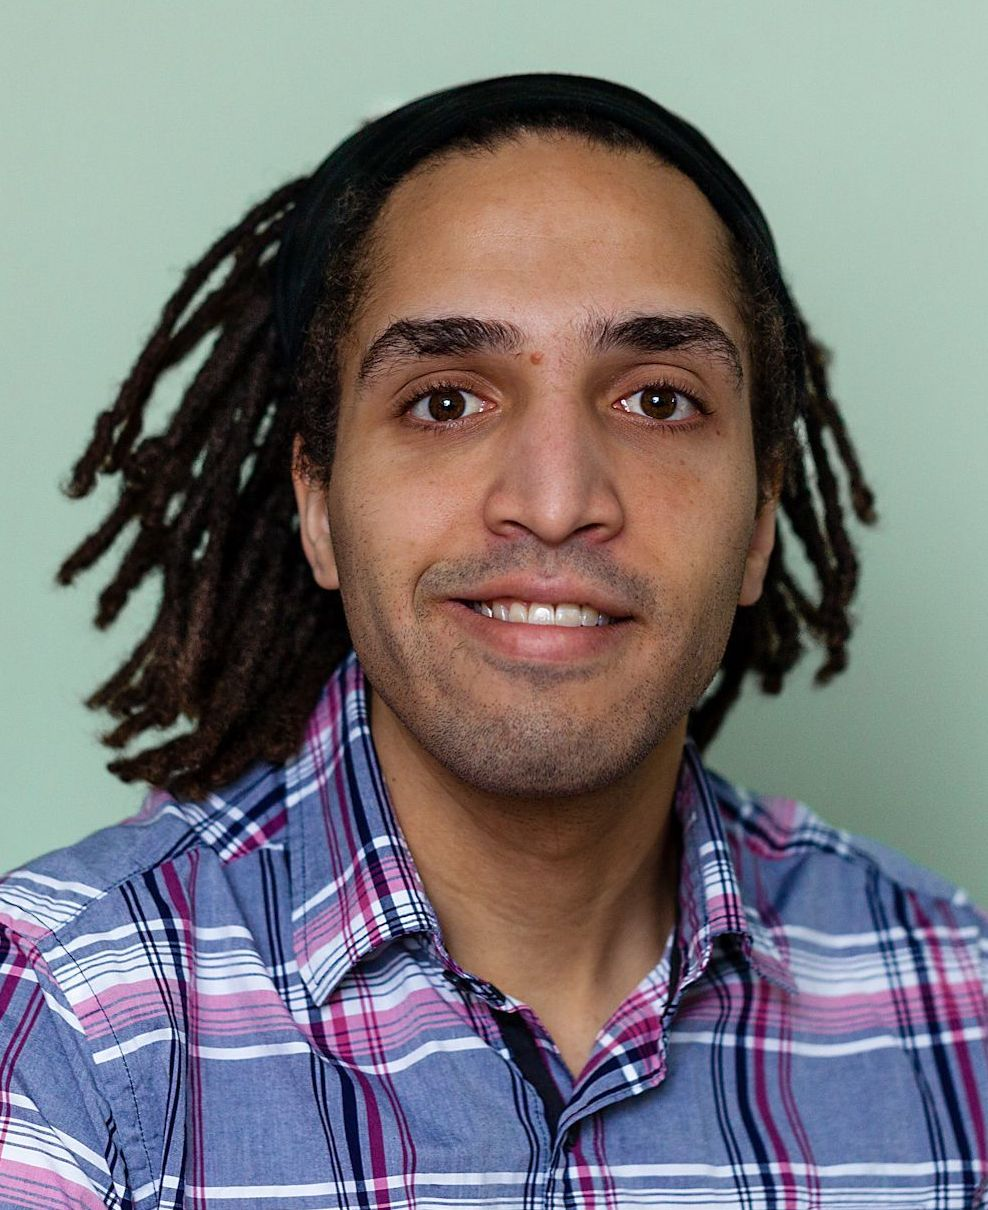
\includegraphics[width=1in,height=1.25in,clip,keepaspectratio]{biopics/shane.jpg}}]{Shane McIntosh}
is an assistant professor in the Department of Electrical and Computer Engineering at McGill University, where he leads the Software Repository Excavation and Build Engineering Labs (Software REBELs). He received his Bachelor's degree in Applied Computing from the University of Guelph and his Master's and PhD in Computer Science from Queen's University, for which he was awarded the Governor General of Canada's Academic Gold Medal. In his research, Shane uses empirical software engineering techniques to study software build systems, release engineering, and software quality. More about Shane and his work is available online at \url{http://rebels.ece.mcgill.ca/}.
\end{IEEEbiography}

\begin{IEEEbiography}[{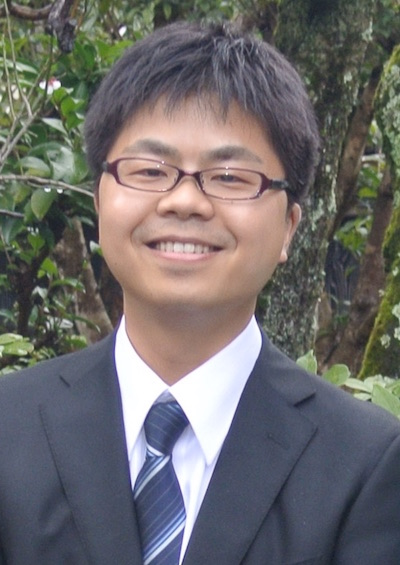
\includegraphics[width=1in,height=1.25in,clip,keepaspectratio]{biopics/yasu.jpg}}]{Yasutaka Kamei}
is an associate professor at Kyushu University in Japan. He has been a research fellow of the JSPS (PD) from July 2009 to March 2010. From April 2010 to March 2011, he was a postdoctoral fellow at Queen’s University in Canada. He received his B.E. degree in Informatics from Kansai University, and the M.E. degree and Ph.D. degree in Information Science from Nara Institute of Science and Technology. His research interests include empirical software engineering, open source software engineering and Mining Software Repositories (MSR). His work has been published at premier venues like ICSE, FSE, ESEM, MSR and ICSM, as well as in major journals like TSE, EMSE, and IST. He will be a program-committee co-chair of the 15th International Conference on Mining Software Repositories (MSR 2018). More information about him is available online at \url{http://posl.ait.kyushu-u.ac.jp/~kamei/}.
\end{IEEEbiography}

\end{document}
